\documentclass[12pt, a4paper, oneside]{article}
\usepackage[left=1in, right=1in]{geometry}
\usepackage[utf8]{inputenc}
\usepackage[T1]{fontenc}
\usepackage{polski}
\usepackage{graphicx}
\usepackage{listings}
\usepackage{cite}
%\usepackage[numbers,sort&compress]{natbib}
\usepackage{notoccite}
\usepackage{multirow}
\usepackage{float}



\usepackage{mathtools, amsthm, amssymb}
\mathtoolsset{showonlyrefs, mathic}

\newtheorem{theorem}{Twierdzenie}
\newtheorem{lemat}{Lemat}
\newtheorem{uwaga}{Uwaga}
\newtheorem{przyklad}{Przykład}
\newtheorem{wniosek}{Wniosek}

\newcommand{\mychapter}[2]{
	\setcounter{chapter}{#1}
	\setcounter{section}{0}
	\chapter*{#2}
	\addcontentsline{toc}{chapter}{#2}
}


\author{Paweł Budzyński \\ Wydział Matematyki, Politechnika Wrocławska}
\title{\textbf{Wykorzystanie sieci neuronowych w problemie wykrywania uszkodzeń lokalnych w maszynach górniczych}}
\date{2018 \\ Październik}

\begin{document}
	\maketitle
	%\tableofcontents
	%\mychapter{1}{Wstęp}
	\section{Wstęp}
	Tematem pracy jest wykorzystanie sieci neuronowych w problemie wykrywania uszkodzeń lokalnych w maszynach górniczych. Zadanie polega na przetworzeniu sygnału diagnostycznego oraz dokonaniu na jego podstawie decyzji o możlwości wystąpienia uszkodzenia w mechanizmach maszyny górniczej.
	
	\subsection{Opis problemu}
	
	Uszkodzenia lokalne są uszkodzeniami występującymi w łożyskach i przekładniach maszyn górniczych. Ich powstawanie uzależnione jest od zmiennych warunków eksploatacyjnych. Uszkodzenie w początkowym stanie obniża sprawność maszyny a ostatecznie może doprowadzić do jej unieruchomienia. Jest to szczególnie problematyczne ponieważ kopalnia dysponuje często jedną lub dwiema takimi maszynami, dodatkowo każda z nich pracuje wyłącznie na swoim stanowisku, nie są one przemieszczane. Detekcja uszkodzenia we wstępnym stadium rozwoju jest ważnym zagadnieniem ponieważ pozwala z wyprzedzeniem określić moment konserwacji urządzenia. 
	
		W detekcji uszkodzeń najczęściej wykorzystuje się diagnostykę wibroakustyczną. Metoda polega na umieszczeniu sensora na obudowie urządzenia, następnie następuje pomiar drgań. Otrzymany sygnał zawiera pewien zakres informacji na podstawie których możemy wnioskować o zaistnieniu uszkodzenia w urządzeniu. W przypadku opisywanych uszkodzeń okazuje się że ich obecność objawia się poprzez pulsacje w sygnale.
	% Sygnał z pulsacjami i bez pulsacji
	
	Jednak w zależności od stopnia uszkodzenia pulsacje mogą mieć różne amplitudy, w przypadku wczesnego stadium rozwoju uszkodzenia najczęściej nie wystaja one ponad poziom szumu.
	Można zatem stwierdzić że detekcja uszkodzenia, z puktu widzenia matematyki, sprowadza się do wykrycia pulsacji. 
	
	%wykrywanie uszkodzeń lokalnych jest jednym z \cite{Zimroz01}
	%Uszkodzenia lokalne powstające w przekładniach kół czerpakowych maszyn górniczych, są to na %przykład ubytki, pęknięcia, wykruszone zęby.  Najskutecznejszą obecnie metodą pozyskania sygnału %jest diagnostyka wibroakustyczna, okazuje się że uszkodzenia takie objawiają się cyklicznymi %pulsacjami w sygnale. Amplituda pulsacji zależy od stopnia uszkodzenia. Z punktu widzenia %matematyki detekcja takiego uszkodzenia polega na wykryciu, zazwyczaj niewidocznych na pierwszy %rzut oka, pulsacji w sygnale diagnostycznym. 
	
	
	\subsection{Sieci neuronowe}
	Sieci neuronowe można zdefiniować jako struktury matematyczne realzujące obliczenia lub przetwarzające sygnały poprzez rzędy elementów zwanych sztucznymi neuronami. \cite{Sieci}
	Sieci neuronowe są jedną z prężnie roziwjających się technologii nauczania maszynowego i szeroko wykorzystywane w pracach nad sztuczną inteligencją.
	Prężny rozwój dziedziny zapoczątkowało wynalezienie sztucznego perceptronu w 1957r.[źródło]. Był to model sztucznego neuronu pozwalającego na binarną klasyfikację liniowo separowalnych danych. Wraz z upływem czasu pojawiaja się kolejne modele neuronów i rodzaje sieci neuronowych. 
	\\
	Chociaż jest to stosunkowo nowa technologia, znalazła już ona szereg zastosowań w wielu dziedzinach. Do najpopularniejszych zastosowań należy przetwarzanie obrazu takie jak rozpoznawanie twarzy, detekcja obiektów, wykrywanie zmian nowotworowych [źródło], przetwarzanie mowy, na przykład w asystentach [źródło] czy też autokorekta i podpowiadanie słów w klawiaturach smartfonów [źródło].
	
	
	
	%\chapter{Metodologia}
	\section{Metodologia}
	
	\subsection{Wstępne przetwarzanie danych}
	
	\subsection{Zastosowanie sieci neuronowych}
	
	\begin{figure}[H]
		\centering
		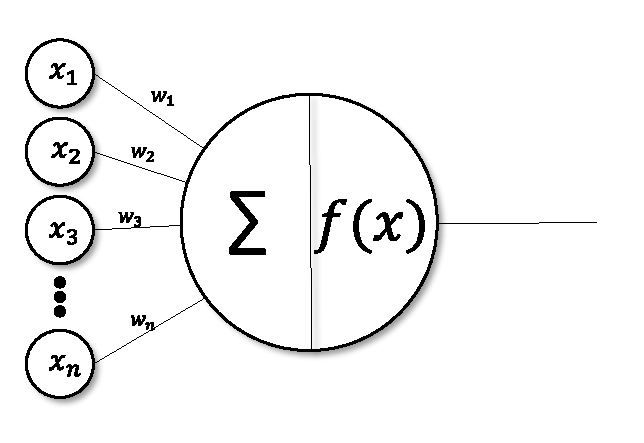
\includegraphics[width=10cm]{images/perceptron_c.pdf}
		\caption{Perceptron}
	\end{figure}
	\begin{figure}[H]
		\centering
		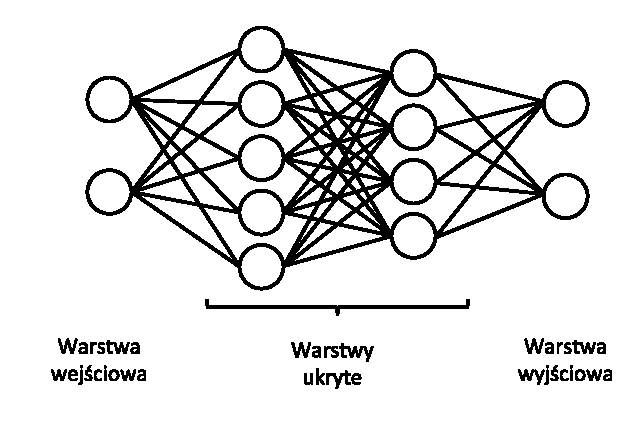
\includegraphics[width=10cm]{images/siec_c.pdf}
		\caption{Perceptron wielowarstwowy}
	\end{figure}
	\begin{figure}[H]
		\centering
		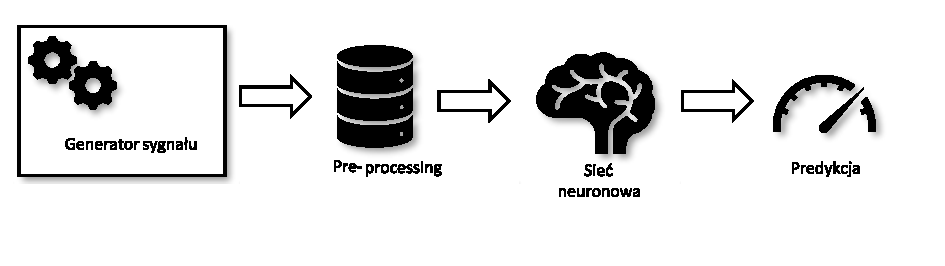
\includegraphics[width=10cm]{images/workflow_c.pdf}
		\caption{Schemat przebiegu pracy systemu wykrywania uszkodzenia}
	\end{figure}
	\begin{figure}[H]
		\centering
		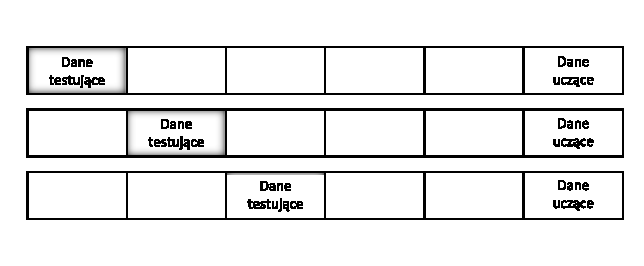
\includegraphics[width=10cm]{images/walidacja_c.pdf}
		\caption{Walidacja krzyżowa}
	\end{figure}
	
	
	% opis dzialania sieci neuronowej jak sadze
	
	
	
	\cite{Wylomanska01}
	
	
	
	%\chapter{Wyniki dla danych symulowanych}
	\section{Projektowanie sieci neuronowej}
	Skuteczność rozwiązania silnie zależy od użytej sieci. Projektowanie sieci polega na doborze tak zwanych hiperparametrów (\textit{ang. hyperparameters}). Zalicza się do nich między innymi:
	\begin{itemize}
		\item Liczba warstw ukrytych
		\item Liczba neuronów w warstwach
		\item Algorytm nauczania oraz jego parametry
		\item Funkcje aktywacji w neuronach.
	\end{itemize}

	Nie istnieje skuteczna metoda doboru parametrów, przy zastowoaniu złożonych sieci badacze najczęściej polegają na swoim doświadczeniu oraz ntuicji. Na potrzeby tego zadania przeprowadzono szereg eksperymentów mających na celu określić najskuteczniejszą sieć do tykonania postawionego zadania. \\
	
	Żeby tego dokonać należy ustalić sposób pomiaru skuteczności danej sieci, w tym celu posłużono się macierzą pomyłek oraz zdefiniowanymi przy jej pomocy miarami.

	\begin{table}[H]
		\begin{tabular}{lccc}
			& \multicolumn{1}{l}{}                    & \multicolumn{2}{c}{\textbf{klasa rzeczywista}}                                                                                                                                      \\ \cline{3-4} 
			& \multicolumn{1}{c|}{}                   & \multicolumn{1}{c|}{\textbf{pozytywna}}                                                  & \multicolumn{1}{c|}{\textbf{negatywna}}                                                  \\ \cline{2-4} 
			\multicolumn{1}{c|}{\multirow{2}{*}{\textbf{klasa predykowana}}} & \multicolumn{1}{c|}{\textbf{pozytywna}} & \multicolumn{1}{c|}{\begin{tabular}[c]{@{}c@{}}prawdziwie\\ pozytywna (TP)\end{tabular}} & \multicolumn{1}{c|}{\begin{tabular}[c]{@{}c@{}}fałszywie\\ pozytywna (FP)\end{tabular}}  \\ \cline{2-4} 
			\multicolumn{1}{c|}{}                                            & \multicolumn{1}{c|}{\textbf{negatywna}} & \multicolumn{1}{c|}{\begin{tabular}[c]{@{}c@{}}fałszywie\\ negatywna (FN)\end{tabular}}  & \multicolumn{1}{c|}{\begin{tabular}[c]{@{}c@{}}prawdziwie\\ negatywna (TN)\end{tabular}} \\ \cline{2-4} 
		\end{tabular}
	\caption{Macierz pomyłek}
	\end{table}

	\begin{center}
		\begin{enumerate}
			\item Dokładność (\textit{ang. accuracy})
			\begin{equation}
				acc = \frac{TP + TN}{P + N}
			\end{equation}
			\item Czułość (\textit{ang. recall}) - odsetek prawdziwie pozytywnych
			\begin{equation}
				recall = \frac{TP}{TP + FN}
			\end{equation}
			\item Precyzja (\textit{ang. precision})
			\begin{equation}
				precision = \frac{TP}{TP + FP}
			\end{equation}
			\item F1 - średnia harmoniczna precyzji i czułości 
			\begin{equation}
				F1 = 2 \cdot \frac{precision \cdot recall}{precision + recall}
			\end{equation}
		\end{enumerate}
		
	\end{center}
	
	Badanie skuteczności sieci opiera się na metodyce walicacji krzyżowej czyli podziału zbioru danych na części a następnie użycie każdej z kolejno do tesowania, reszta do uczenia <- to do metodyki
	

	\subsection{Zależność od danych wejściowych}
	Pierwszy eksperyment będzie postawą do decyzji o tym jakich danych należy użyć do uczenia sieci. Należy porównać jak uczy się sieć w zależności od danych wejściowych. Porównane zostaną dwa podejścia: użycie surowego sygnału oraz wstępnie przetworzonego. 
	
	\begin{enumerate}
		\item Surowy sygnał podeście pierwsze
			\subitem dane wejściowe: 4096
			\subitem warstwy ukryte: 1000 - 500 - 200
			\subitem liczba wag: 
		
		\item Surowy sygnał podejście drugie
			\subitem dane wejściowe: 4096
			\subitem warstwy ukryte: 500 - 200
			\subitem liczba wag:
			
		\item Estymatory sygnału
			\subitem dane wejściowe: 8
			\subitem warstwy ukryte: 5 - 3 - 2
			\subitem liczba wag: mało
	\end{enumerate}
	
	Wyniki eksperymentu prezentują sie następująco.
	

	\begin{figure}[H]
		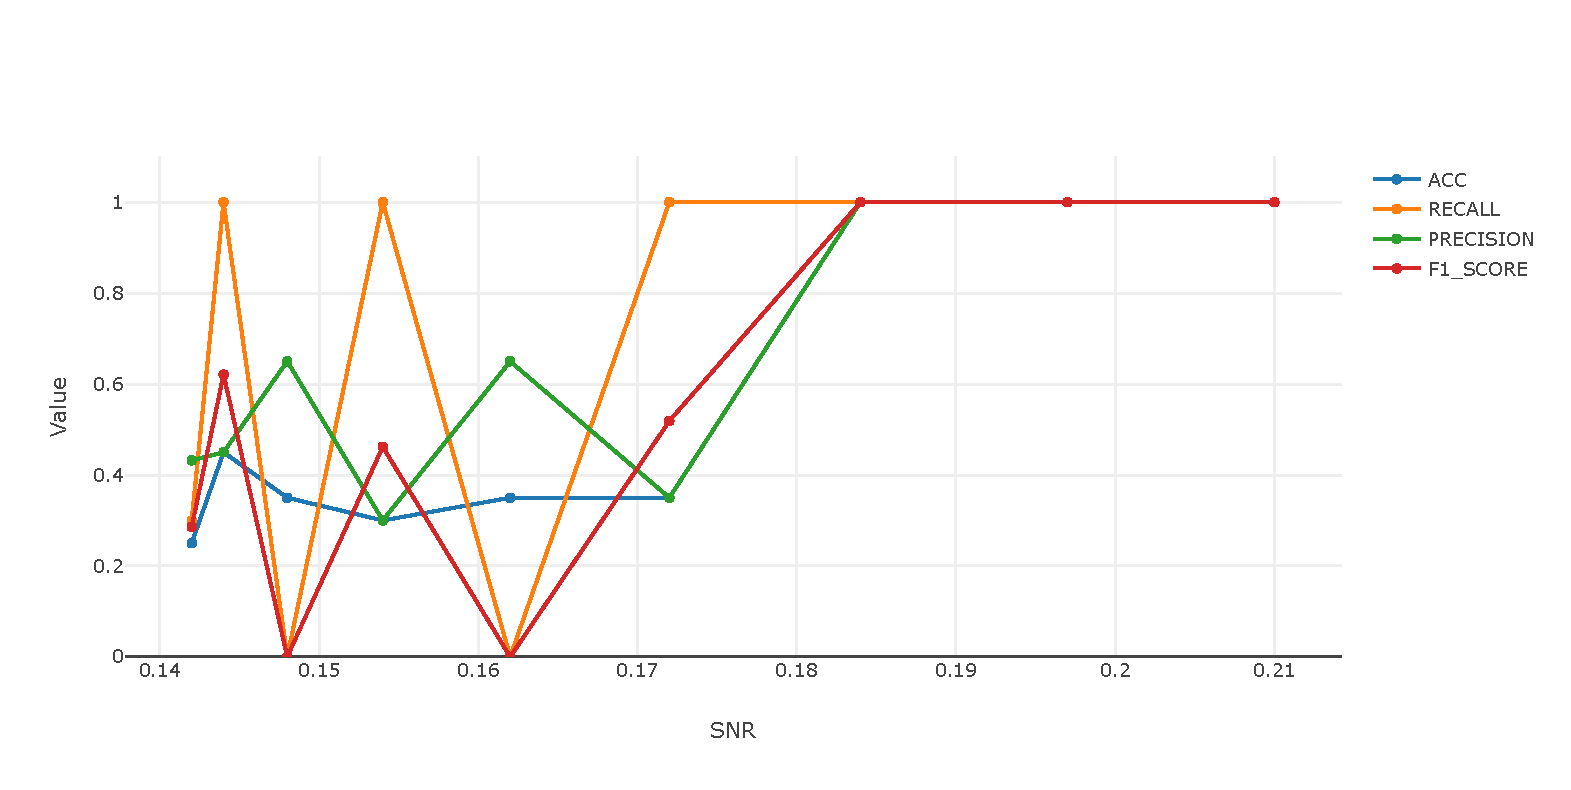
\includegraphics[width=16cm]{images/nn_full_1000_500_200.pdf}
		\caption{Wyniki surowego sygnału, architektura -1000-500-200-}
	\end{figure}

	\begin{figure}[H]
		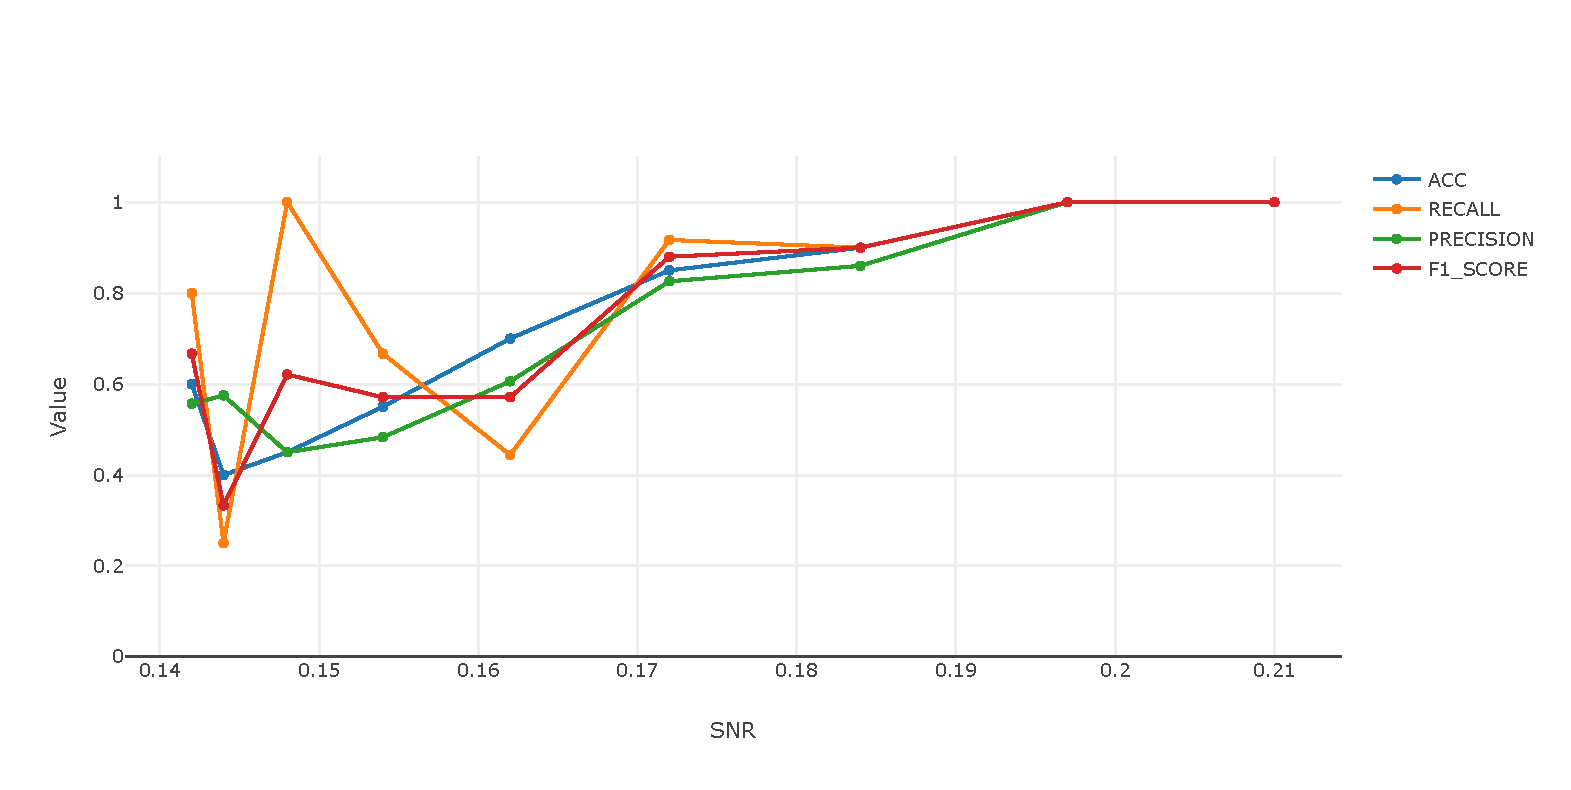
\includegraphics[width=16cm]{images/nn_full_signal_500_200.pdf}
		\caption{Wyniki dla surowego sygnału, architektura -500-200-}
	\end{figure}

	\begin{figure}[H]
		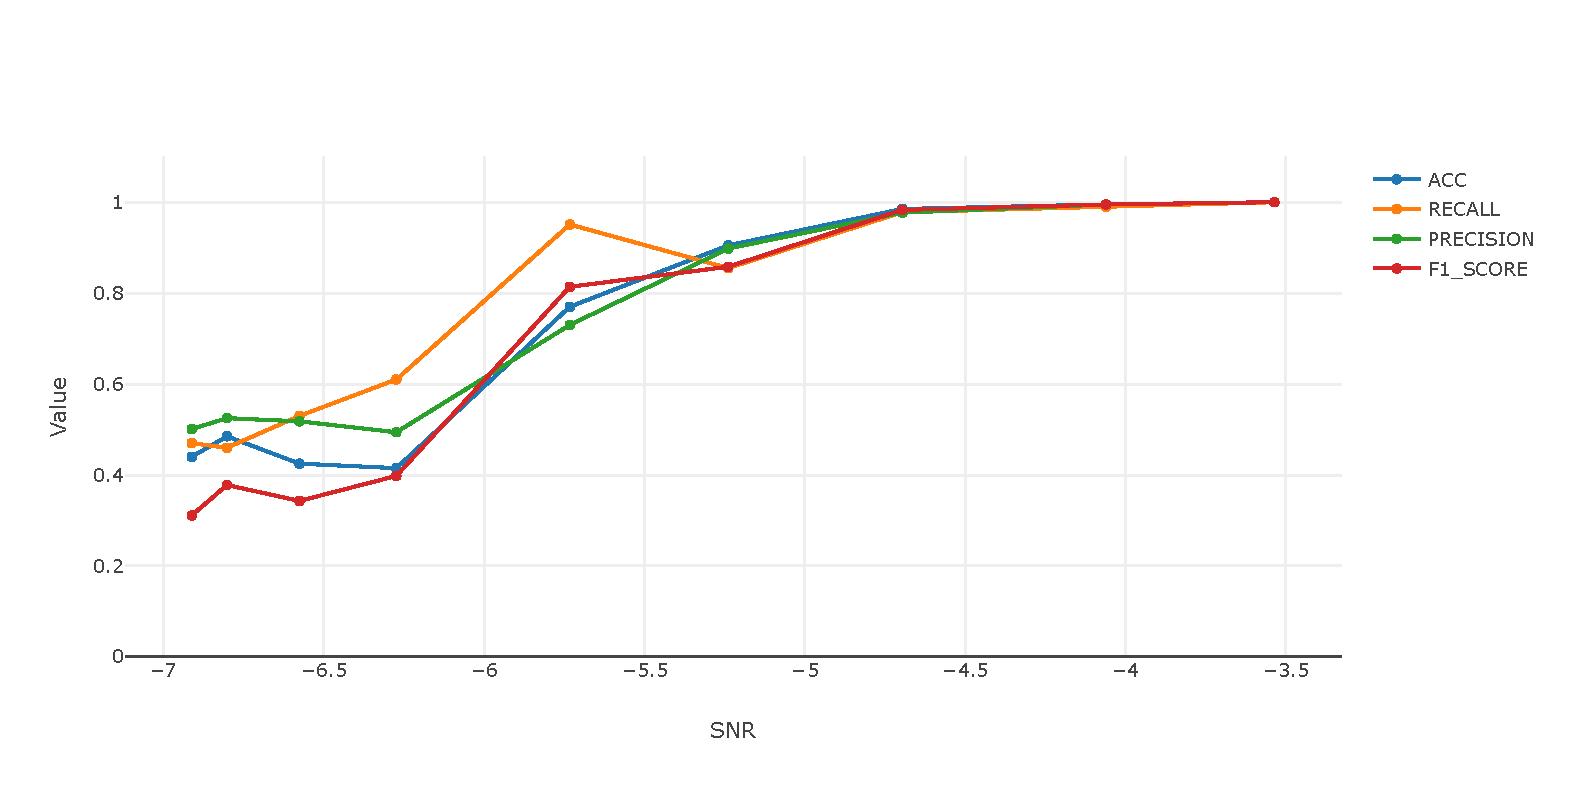
\includegraphics[width=16cm]{images/nn_small_532.pdf}
		\caption{Wyniki dla estymatorów, architektura -5-3-2-}
	\end{figure}

	Zastosowanie surowego sygnału, niezależnie od architektury, daje bardzo chaotyczne wyniki sugerujące że proces nauczania nie przebiega prawidłowo a predykcja jest obarczona dużym błędem. Podejście z zastosowaniem surowego sygnału jest kosztowne obliczeniowo i mało efektywne dlatego należy je wykluczyć z dalszych roważań. Z kolei zastosowanie estymatórów opisujących sygnał daje obiecujące wyniki pozwalające wnioskować o skutecznym uczeniu się sieci. W oparciu o zaproponowaną architekturę zostanie przeprowadzony kolejny eksperyment mający stwierdzić czy przy użyciu obecnych danych uczących można otrzymać lepsze wyniki.
	
	\subsection{Zależność od architektury}
	Po decyzji o użyciu estymatorów jako danych uczących należy przeprowadzić eksperyment mający na celu określenie najlepszej architektury sieci neuronowej. Ponieważ architektura zaproponowana w poprzednim eksperymencie dawała wyniki świadczące o poprawnie przebiegającym procesie uczenia zaproponowano różne jej wariancje. 
		\begin{figure}[H]
		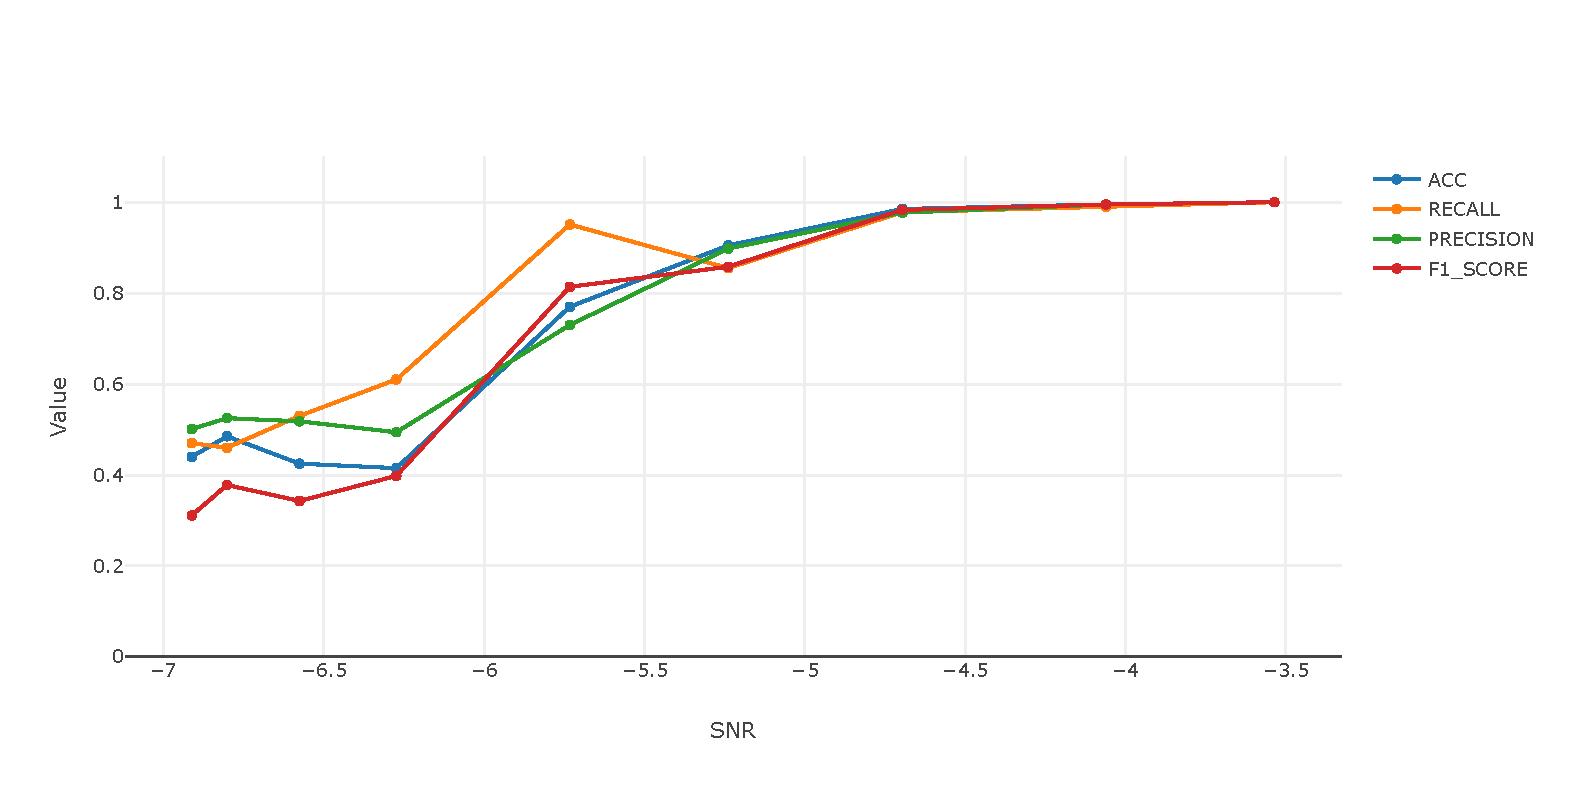
\includegraphics[width=16cm]{images/nn_small_532.pdf}
		\caption{Wyniki dla sieci o architekturze -5-3-2-}
	\end{figure}
	\begin{figure}[H]
		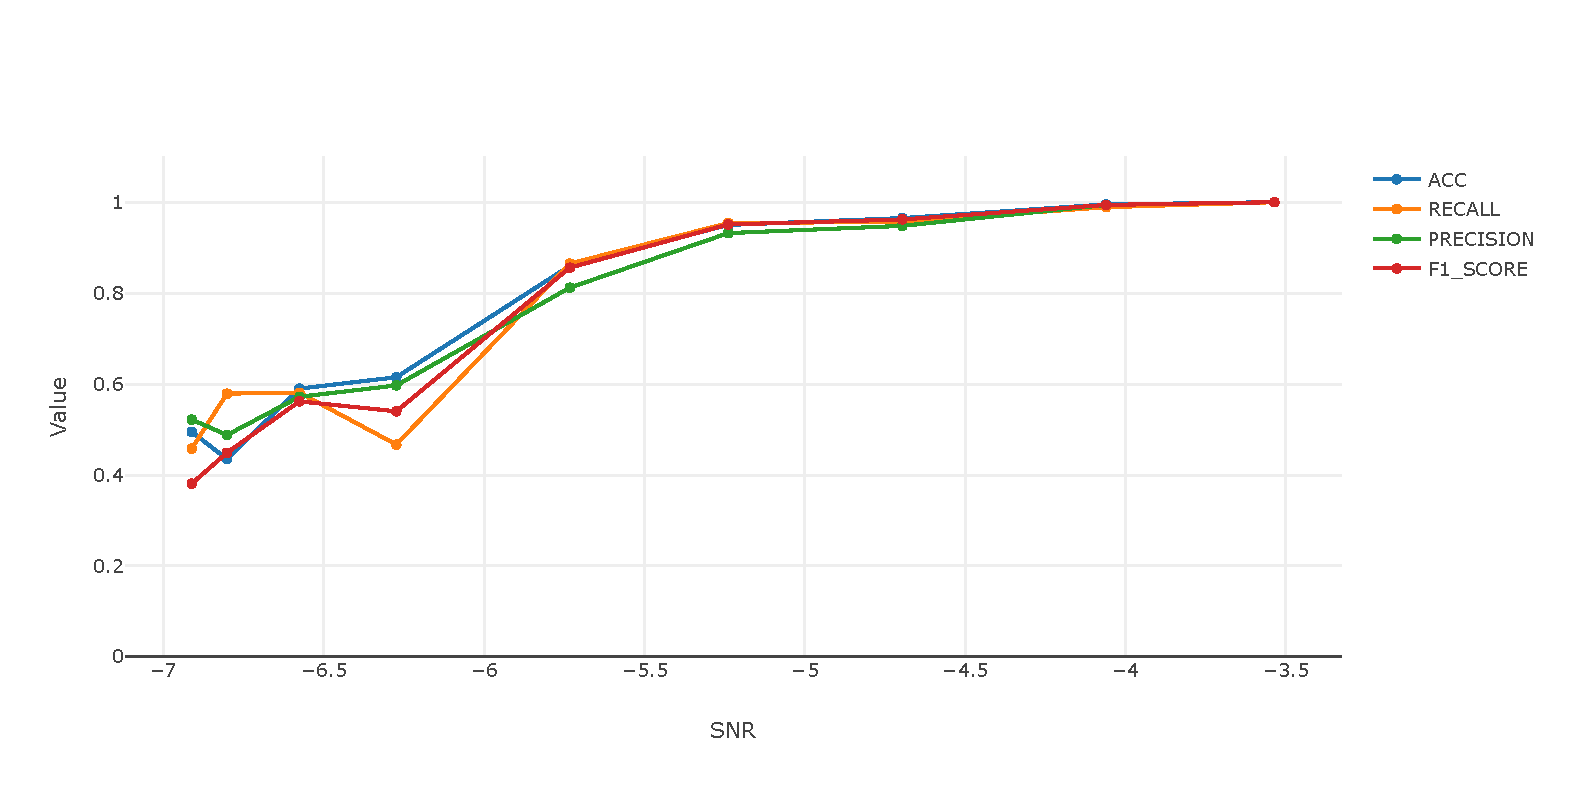
\includegraphics[width=16cm]{images/nn_small_85.pdf}
		\caption{Wyniki dla sieci o architekturze -8-5-}
	\end{figure}
		\begin{figure}[H]
			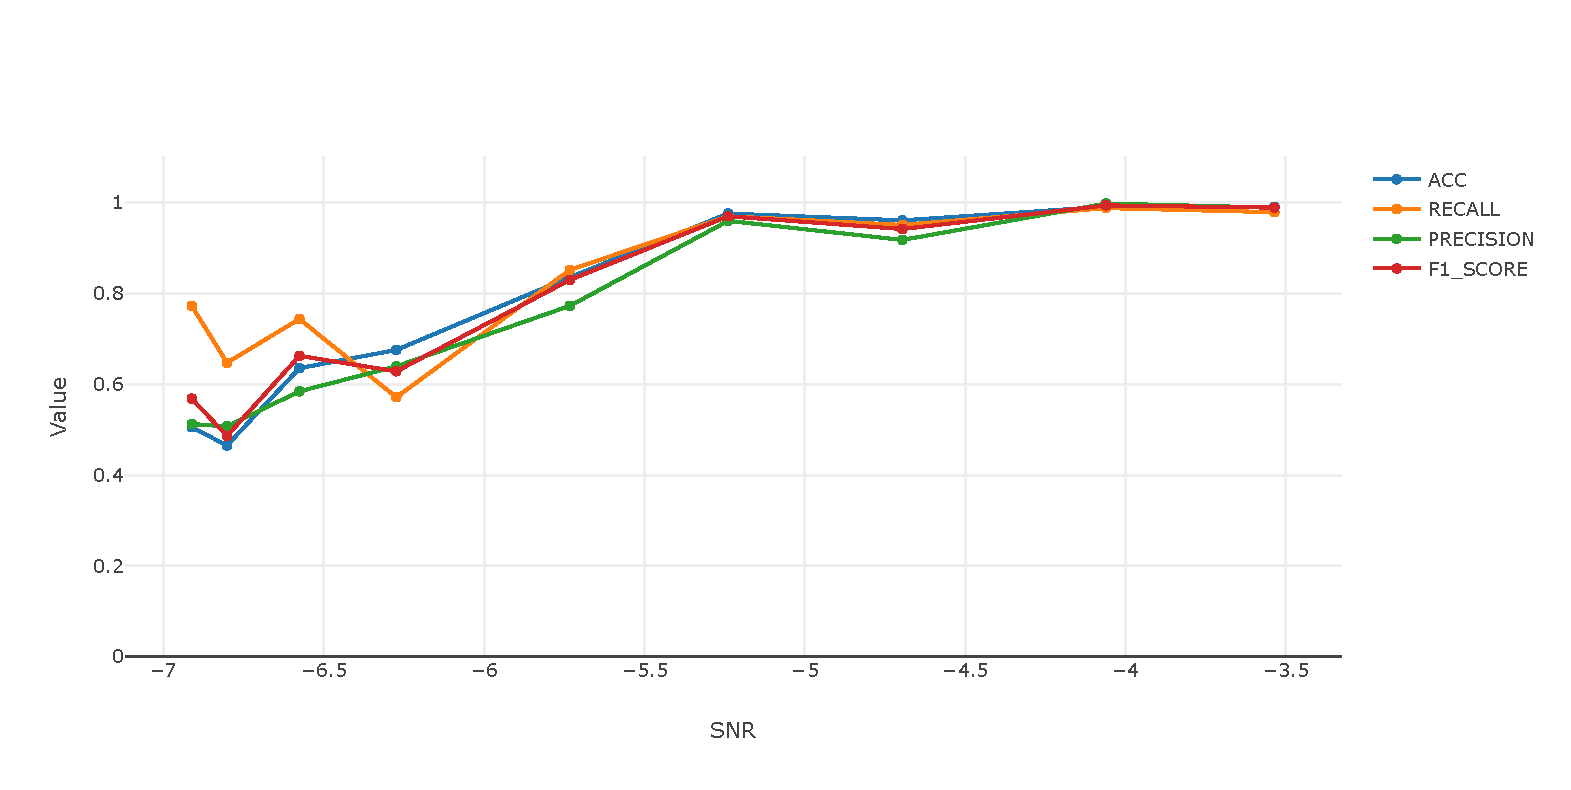
\includegraphics[width=16cm]{images/nn_small_2.pdf}
			\caption{Wyniki dla sieci o architekturze -2-}
		\end{figure}
	\begin{figure}[H]
		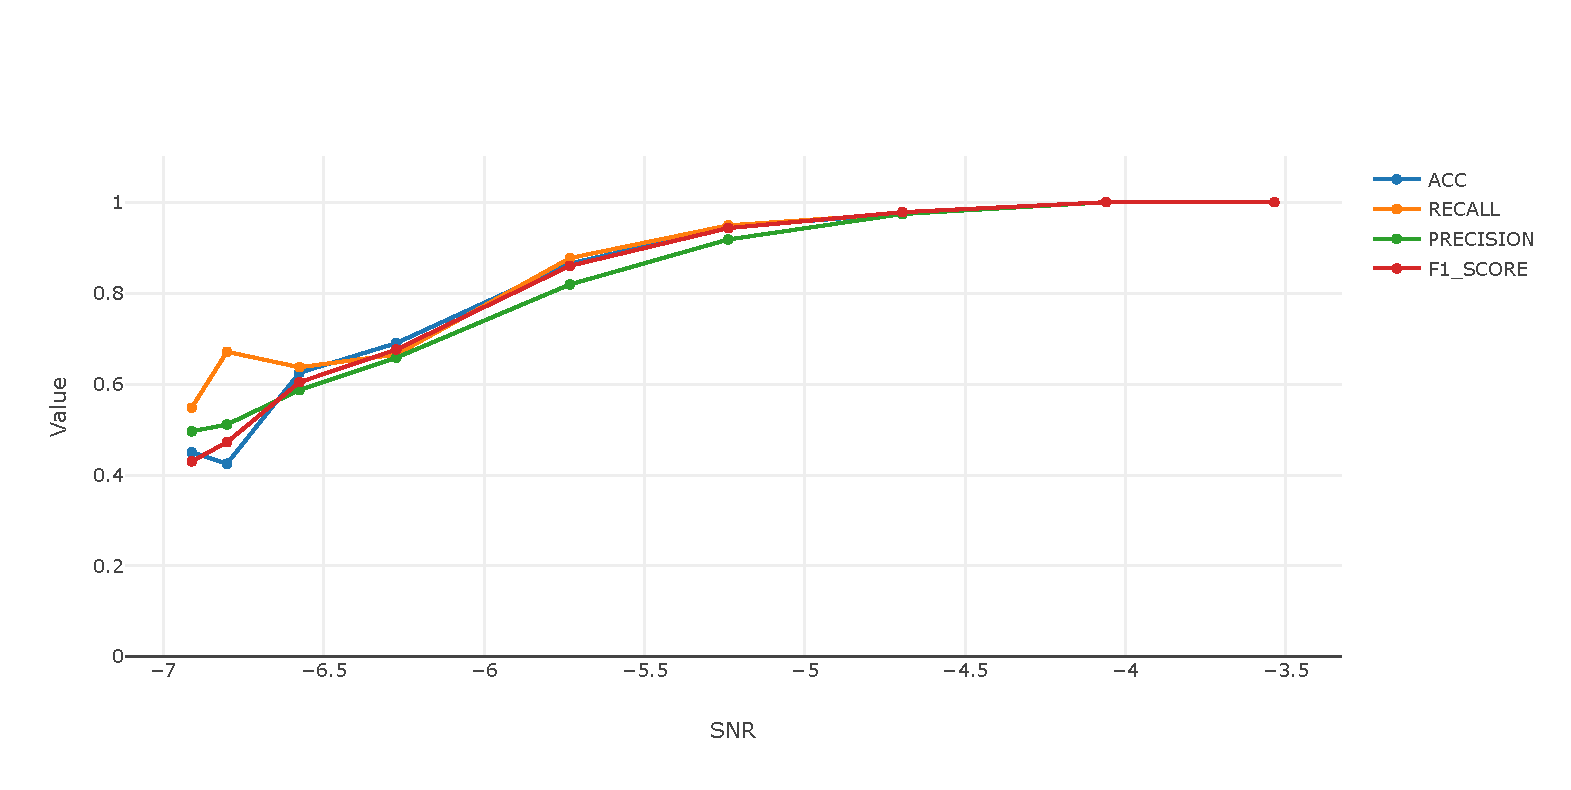
\includegraphics[width=16cm]{images/nn_small_5.pdf}
		\caption{Wyniki dla sieci o architekturze -5-}
	\end{figure}


	
	
	%Nauczanie sieci 
	%Z powodu zapotrzebowania na dużą ilosć danych w procesie uczenia sieci neuronowych dalsza praca opiera się na danych symulowanych. Program generujący sygnał pozwala na dobór szeregu parametrów takich jak częstotliwości, amplitudy, zaszumienie oraz siłę pulsacji.
	%\subsection{Przygotowanie danych}
	%Przed przystąpieniem do uczenia należało przygotować dane uczące, w tym przypadku jest to zestaw sygnałów bez pulsacji oraz sygnałów z różnymi pulsacjami, poniżej przedstawiono tabelkę szczegółowo opisującą przygotowany zbiór danych.
	%\subsection{Surowy sygnał}
	%Pierwszym eksperymentem było przetestowanie jak sieć poradzi sobie w przypadku surowych danych. Do nauczania użyto sygnału odpowiadającemu jednej sekundzie odczytu, co przy próbkowaniu na poziomie $x$ daje $w chuj$ próbek.
	%\\ Tutaj jebniesz schemat sieci
	%\\A tutaj tabelka z wniami 
	%Eksperyment ten przeprowadzony był bardziej dla porównania niż z żeczywistej potrzeby, użycie surowego sygnału i takiej ilości próbek nie wydaje się był optymalnym rozwiązaniem za to jest kosztowne, dobrą praktyką w dziedzinie nauczania maszynowego jest wstępna obróbka danych i znalezienie sposobu na 

	\subsection{Estymatory}
	
	%\chapter{Wnioski}
	\section{Wnioski}
	
	
	
	\begin{center}
		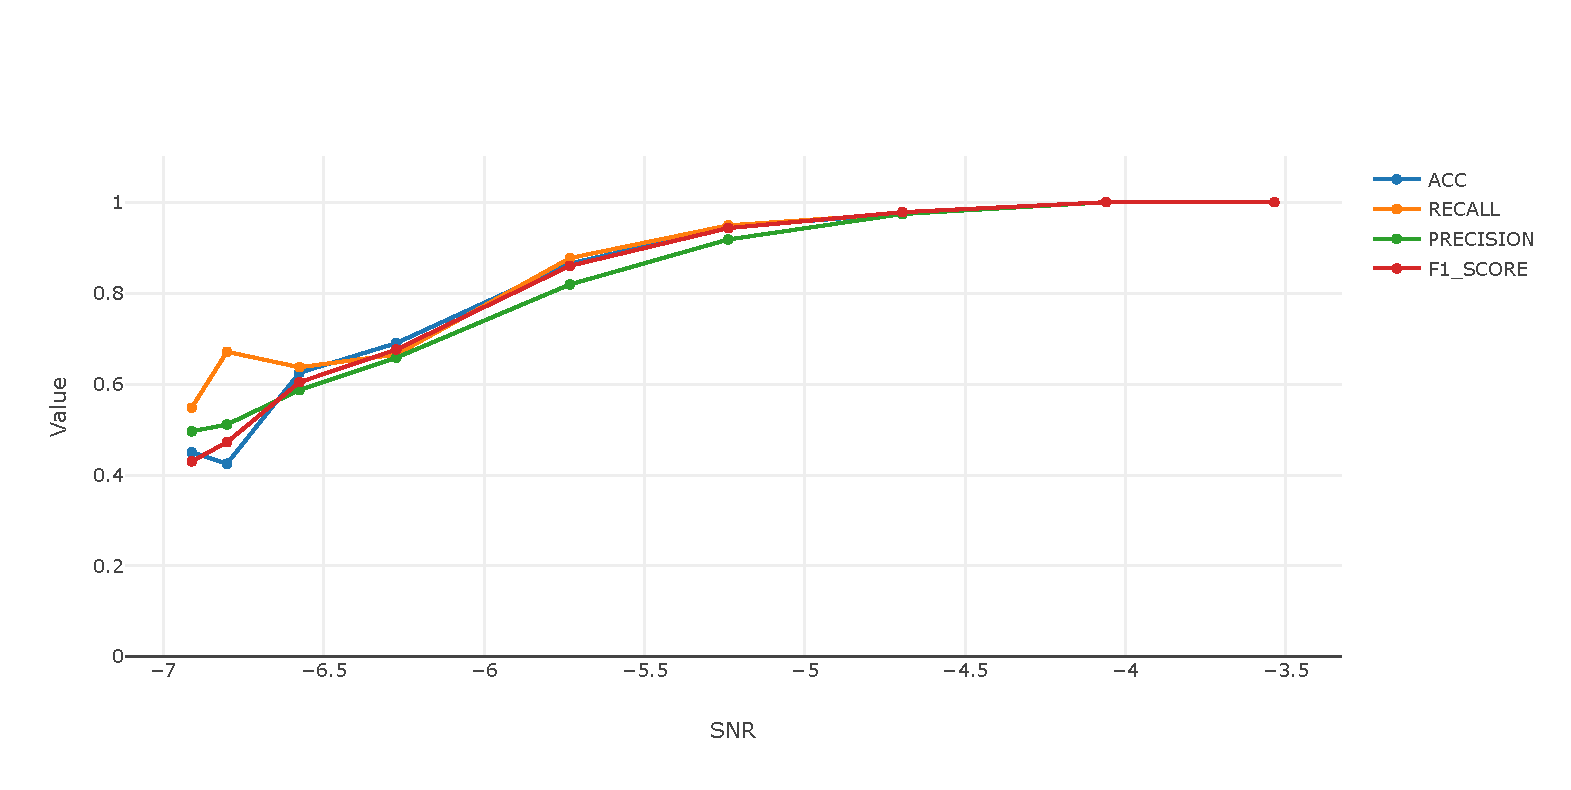
\includegraphics[width=16cm]{images/nn_small_5.pdf}
	\end{center}
	
	
	%\bibliographystyle{unsrt}
	\bibliography{mybib}
\end{document}